% ============================================================
%  GAME DESIGN DOCUMENT — Robot Programmer (CodeBot Maze)
% ============================================================
\documentclass[12pt,a4paper]{article}

% ── Packages ────────────────────────────────────────────────
\usepackage[a4paper, margin=2.5cm]{geometry}
\usepackage[T1]{fontenc}
\usepackage[utf8]{inputenc}
\usepackage{lmodern}
\usepackage{microtype}
\usepackage{xcolor}
\usepackage{graphicx}
\usepackage{tikz}
\usetikzlibrary{shapes.geometric, arrows.meta, positioning, calc, fit, backgrounds, shadows}
\usepackage{pgfplots}
\pgfplotsset{compat=1.18}
\usepackage{listings}
\usepackage{booktabs}
\usepackage{tabularx}
\usepackage{longtable}
\usepackage{array}
\usepackage{enumitem}
\usepackage{fancyhdr}
\usepackage{titlesec}
\usepackage{tcolorbox}
\tcbuselibrary{skins, breakable, listingsutf8}
\usepackage{hyperref}
\usepackage{amsmath}
\usepackage{amssymb}
\usepackage{float}
\usepackage{caption}
\usepackage{subcaption}
\usepackage{mdframed}
\usepackage{multicol}
% \usepackage{fontawesome5}  % removed: not available on all TeX distributions

% ── Colour palette ───────────────────────────────────────────
\definecolor{primary}{HTML}{2B3A67}
\definecolor{accent}{HTML}{E84855}
\definecolor{lightblue}{HTML}{87CEEB}
\definecolor{darkbg}{HTML}{161620}
\definecolor{codebg}{HTML}{16161F}
\definecolor{codefg}{HTML}{B4F0B4}
\definecolor{keyword}{HTML}{7FAAFF}
\definecolor{number}{HTML}{FFD700}
\definecolor{comment}{HTML}{6A9955}
\definecolor{sectionbg}{HTML}{E8EEF8}
\definecolor{accentlight}{HTML}{FDE8EA}
\definecolor{gridbg}{HTML}{F0F4FF}

% ── Section formatting ───────────────────────────────────────
\titleformat{\section}
  {\Large\bfseries\sffamily\color{primary}}
  {\colorbox{primary}{\color{white}\thesection}}
  {0.5em}
  {}
  [{\color{primary}\rule{\linewidth}{2pt}}\vspace{2pt}]

\titleformat{\subsection}
  {\color{primary}\large\bfseries\sffamily}
  {\thesubsection}
  {0.5em}
  {}
  [{\color{accent}\rule{\linewidth}{1.5pt}}\vspace{2pt}]

\titleformat{\subsubsection}
  {\color{primary}\normalsize\bfseries\sffamily}
  {\thesubsubsection}
  {0.5em}
  {}

% ── Header / footer ─────────────────────────────────────────
\pagestyle{fancy}
\fancyhf{}
\fancyhead[L]{\color{primary}\sffamily\bfseries Robot Programmer — GDD}
\fancyhead[R]{\color{primary}\sffamily CodeBot Maze}
\fancyfoot[C]{\color{primary}\thepage}
\renewcommand{\headrulewidth}{1.5pt}
\renewcommand{\headrule}{\hbox to\headwidth{\color{primary}\leaders\hrule height \headrulewidth\hfill}}

% ── tcolorbox styles ─────────────────────────────────────────
\tcbset{
  gddbox/.style={
    enhanced, breakable,
    colback=sectionbg, colframe=primary,
    fonttitle=\bfseries\sffamily\color{white},
    coltitle=white, attach boxed title to top left={yshift=-2mm, xshift=4mm},
    boxed title style={colback=primary, rounded corners},
    arc=3pt, outer arc=3pt,
    left=6pt, right=6pt, top=10pt, bottom=6pt
  },
  redbox/.style={
    enhanced, breakable,
    colback=accentlight, colframe=accent,
    fonttitle=\bfseries\sffamily\color{white},
    coltitle=white, attach boxed title to top left={yshift=-2mm, xshift=4mm},
    boxed title style={colback=accent, rounded corners},
    arc=3pt, outer arc=3pt,
    left=6pt, right=6pt, top=10pt, bottom=6pt
  },
  codebox/.style={
    enhanced, breakable,
    colback=codebg, colframe=primary!60,
    fonttitle=\bfseries\sffamily\color{white},
    coltitle=white,
    attach boxed title to top left={yshift=-2mm, xshift=4mm},
    boxed title style={colback=primary!80!black, rounded corners},
    arc=3pt, outer arc=3pt,
    left=6pt, right=6pt, top=10pt, bottom=6pt
  }
}

% ── Code listings ────────────────────────────────────────────
\lstdefinelanguage{RobotScript}{
  morekeywords={moveUp, moveDown, moveLeft, moveRight, repeat, end},
  sensitive=false,
  morecomment=[l]{//},
  morestring=[b]"
}

\lstset{
  language=RobotScript,
  basicstyle=\ttfamily\small\color{codefg},
  keywordstyle=\color{keyword}\bfseries,
  numberstyle=\tiny\color{gray},
  stringstyle=\color{number},
  commentstyle=\color{comment}\itshape,
  numbers=left,
  numbersep=8pt,
  frame=none,
  backgroundcolor=\color{codebg},
  breaklines=true,
  showstringspaces=false,
  tabsize=2,
  xleftmargin=16pt
}

\lstdefinelanguage{EBNF}{
  morekeywords={},
  sensitive=false,
  morestring=[b]",
  morestring=[b]'
}

\lstdefinestyle{ebnf}{
  language={},
  basicstyle=\ttfamily\small\color{white},
  backgroundcolor=\color{primary!90!black},
  breaklines=true, frame=none,
  xleftmargin=10pt, numbers=none,
  showstringspaces=false
}

\lstdefinestyle{java}{
  language=Java,
  basicstyle=\ttfamily\footnotesize\color{codefg},
  keywordstyle=\color{keyword}\bfseries,
  numberstyle=\tiny\color{gray},
  commentstyle=\color{comment}\itshape,
  stringstyle=\color{number},
  numbers=left, numbersep=8pt,
  frame=none, backgroundcolor=\color{codebg},
  breaklines=true, tabsize=2, xleftmargin=16pt
}

% ── Helper commands ──────────────────────────────────────────
\newcommand{\keyword}[1]{\textcolor{keyword}{\texttt{\bfseries #1}}}
\newcommand{\token}[1]{\textcolor{accent}{\texttt{#1}}}
\newcommand{\nonterminal}[1]{\textit{\textcolor{primary}{#1}}}
\newcommand{\gddfield}[2]{%
  \noindent\begin{tabularx}{\linewidth}{>{\bfseries\color{accent}\sffamily}p{3.5cm} X}
    #1 & #2
  \end{tabularx}\smallskip}

% ── Hyperref setup ───────────────────────────────────────────
\hypersetup{
  colorlinks=true,
  linkcolor=primary,
  urlcolor=accent,
  pdfauthor={Team},
  pdftitle={Robot Programmer — Game Design Document},
}

% ============================================================
\begin{document}

% ── Title Page ───────────────────────────────────────────────
\begin{titlepage}
  \pagecolor{primary}
  \color{white}
  \centering
  \vspace*{2cm}

  {\sffamily\Huge\bfseries ROBOT PROGRAMMER}\\[0.4cm]
  {\sffamily\Large\color{lightblue} CodeBot Maze}\\[1.5cm]

  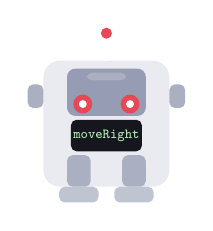
\begin{tikzpicture}
    % Robot body
    \fill[white!90!primary, rounded corners=6pt] (-0.8,-0.8) rectangle (0.8,0.8);
    \fill[primary!50!white, rounded corners=3pt] (-0.5,0.1) rectangle (0.5,0.7);
    \fill[accent] (-0.3,0.25) circle (0.12);
    \fill[accent] (0.3,0.25) circle (0.12);
    \fill[white] (-0.3,0.25) circle (0.05);
    \fill[white] (0.3,0.25) circle (0.05);
    \fill[primary!40!white, rounded corners=2pt] (-0.25,0.55) rectangle (0.25,0.65);
    % Antenna
    \draw[white, line width=1.5pt] (0,0.8) -- (0,1.1);
    \fill[accent] (0,1.15) circle (0.07);
    % Arms
    \fill[primary!40!white, rounded corners=2pt] (-1.0,0.2) rectangle (-0.8,0.5);
    \fill[primary!40!white, rounded corners=2pt] (0.8,0.2) rectangle (1.0,0.5);
    % Legs
    \fill[primary!40!white, rounded corners=2pt] (-0.5,-0.8) rectangle (-0.2,-0.4);
    \fill[primary!40!white, rounded corners=2pt] (0.2,-0.8) rectangle (0.5,-0.4);
    % Feet
    \fill[primary!30!white, rounded corners=2pt] (-0.6,-1.0) rectangle (-0.1,-0.8);
    \fill[primary!30!white, rounded corners=2pt] (0.1,-1.0) rectangle (0.6,-0.8);
    % Chest panel
    \fill[codebg, rounded corners=2pt] (-0.45,-0.35) rectangle (0.45,0.05);
    \node[font=\ttfamily\tiny, text=codefg] at (0,-0.15) {moveRight};
  \end{tikzpicture}

  \vspace{1.5cm}

  {\sffamily\large\bfseries GAME DESIGN DOCUMENT}\\[0.3cm]
  {\sffamily\normalsize Version 1.0 \quad|\quad May 2026}

  \vspace{2cm}

  
\begin{tikzpicture}
    \node[fill=white!10!primary, rounded corners=6pt,
          inner sep=12pt, text width=10cm, align=center] {
      \color{lightblue}\sffamily\bfseries Robot Programmer (CodeBot Maze)\\[4pt]
      \color{white}\sffamily A Serious Game for Computer Science Education\\[4pt]
      \color{lightblue}\sffamily\small University of Macedonia — Master's in Serious Game Development
    };
  \end{tikzpicture}

  \vfill
  \color{white!60!primary}\sffamily\small
  Built with Greenfoot 3 $\cdot$ Java $\cdot$ Custom Programming Language DSL
\end{titlepage}
\pagecolor{white}\color{black}

% ── Table of Contents ────────────────────────────────────────
\tableofcontents
\newpage

% ============================================================
\section{Team Information}
% ============================================================

\begin{tcolorbox}[gddbox, title={Team Details}]
\begin{tabularx}{\linewidth}{>{\bfseries\sffamily\color{primary}}p{4cm} X}
  Team Name   & \textit{[Team Name]} \\[4pt]
  Team Code   & \textit{[Team Code]} \\[4pt]
  \midrule
  Team Captain (\#1) & \textit{[Name]} \\[4pt]
  Team Member \#2    & \textit{[Name]} \\[4pt]
  Team Member \#3    & \textit{[Name]} \\[4pt]
  Team Member \#4    & \textit{[Name]} \\[4pt]
  \midrule
  Institution & University of Macedonia \\[4pt]
  Programme   & Master's in Serious Game Development \\[4pt]
  Academic Year & 2025--2026 \\
\end{tabularx}
\end{tcolorbox}

% ============================================================
\section{Game Overview}
% ============================================================

% ── Game Title ──────────────────────────────────────────────
\begin{tcolorbox}[gddbox, title={Game Title}]
\gddfield{Title:}{\textbf{\Large Robot Programmer} \quad\small(\textit{working subtitle: CodeBot Maze})}

\vspace{6pt}
\gddfield{Why this name?}{%
The name immediately conveys the two core activities: \emph{robots} (the visual, physical agent the player controls) and \emph{programming} (the activity used to control it). Players of any age instantly understand they will write code to move a robot. The subtitle \emph{CodeBot Maze} reinforces the puzzle-navigation structure. The name requires no prior STEM knowledge to make sense, making it accessible to newcomers while accurately describing the learning objective.
}
\end{tcolorbox}

\vspace{6pt}

% ── Game Description ────────────────────────────────────────
\begin{tcolorbox}[gddbox, title={Game Description}]
\textbf{Robot Programmer} is a \emph{serious educational puzzle game} that teaches the foundations of imperative programming and algorithmic thinking through direct play. The player is cast as a robot programmer whose job is to write short programs, in a simple custom scripting language, to guide a robot through increasingly complex grid-based mazes.

\vspace{6pt}
Each level presents a maze populated with \textbf{walls}, \textbf{obstacles}, and a glowing \textbf{goal tile}. The player opens an embedded code editor and types movement commands — \keyword{moveUp}, \keyword{moveDown}, \keyword{moveLeft}, \keyword{moveRight} — and loops — \keyword{repeat}\texttt{(N) \ldots end} — to chart a path from the robot's starting square to the goal. Pressing \textbf{RUN} causes the program to be lexed, parsed, and executed step-by-step on screen: the robot animates one tile per instruction, logging every action to an output terminal below the maze.

\vspace{6pt}
\textbf{Kind of game:} 2D top-down puzzle / coding game (serious game / edugame).\\
\textbf{Who it is for:} Students aged 10--18 with no prior programming experience; also suitable for early university introductory computing courses.
\end{tcolorbox}

\vspace{6pt}

% ── Audience ────────────────────────────────────────────────
\begin{tcolorbox}[gddbox, title={Audience}]
\gddfield{Primary audience:}{Students aged 10--18 in secondary school STEM classes, or first-year university computing students.}
\gddfield{Secondary audience:}{Teachers and educators looking for a classroom demonstration tool for introductory programming concepts.}
\gddfield{Age suitability:}{Rated \textbf{G} (General). All content is abstract and educational — no violence, no mature themes.}
\gddfield{How shown:}{%
  \textbf{(a)} Grid-based visuals at the complexity level of a puzzle game rather than an action game, keeping cognitive load low.
  \textbf{(b)} The scripting language has only six keywords, eliminating syntax complexity common in real languages.
  \textbf{(c)} An in-game instructions screen explains every keyword with worked examples before the player starts.
  \textbf{(d)} Error messages in the terminal are plain English (e.g.\ ``Line 3: Unknown keyword `moveleft2'\,'') rather than cryptic compiler output.
}
\end{tcolorbox}

\vspace{6pt}

% ── Characters / Roles ──────────────────────────────────────
\begin{tcolorbox}[gddbox, title={Characters / Roles}]
\gddfield{Subject:}{The game is about a programmable robot navigating procedurally arranged grid mazes. The story is minimalist — the focus is the programming challenge, not narrative.}

\vspace{4pt}
\begin{tabularx}{\linewidth}{>{\bfseries\color{accent}\sffamily}p{3cm} X}
  \toprule
  Character & Description \\
  \midrule
  \textbf{RIVETS} (the Robot) &
    The player's avatar. RIVETS is a small, friendly-looking robot rendered on a 20\,px grid. It has a distinct visual design (round eyes, antenna, chunky arms/legs) to give it personality without distracting from gameplay. RIVETS responds to every executed instruction with smooth one-tile animation and a terminal log message. It collides with obstacles and cannot pass through walls. \\[6pt]
  \textbf{The Programmer} (player) &
    The player takes the role of the programmer: the unseen human writing code in the editor panel. There is no avatar for this role — the player's presence is expressed through the code they write. This reinforces the real-world relationship between programmer and executing machine. \\[6pt]
  \textbf{Goal} &
    A visually distinct golden star tile that RIVETS must reach. It has no AI or behaviour — it is a static destination object. \\[6pt]
  \textbf{Obstacle} &
    Solid dark blocks that block RIVETS's movement. When RIVETS tries to enter an obstacle tile, the move is cancelled and the terminal logs \texttt{[!] Blocked by obstacle}. \\
  \bottomrule
\end{tabularx}

\vspace{4pt}
\gddfield{Motivations:}{%
RIVETS's ``motivation'' is mechanical: it executes the program literally. This is intentional — a recurring teaching moment is that computers do exactly what you tell them, not what you \emph{meant}. Players quickly learn precision and planning when RIVETS walks into a wall because of a typo.
}
\end{tcolorbox}

\vspace{6pt}

% ── Environment ─────────────────────────────────────────────
\begin{tcolorbox}[gddbox, title={Environment}]
\gddfield{Setting:}{A grid-based 2D maze world rendered in an 800$\times$600-pixel Greenfoot window. Levels take place in an abstract ``robot workshop'' aesthetic — clean lines, minimal decoration, emphasis on readability.}

\vspace{4pt}
\gddfield{Layout:}{The game window is divided into four fixed regions:}

\vspace{4pt}
\begin{center}
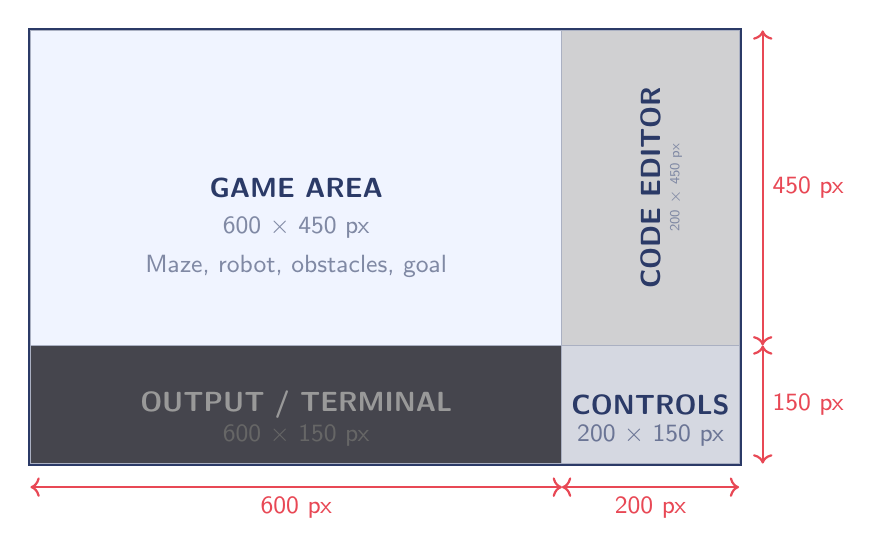
\begin{tikzpicture}[font=\small\sffamily]
  \draw[primary, line width=2pt] (0,0) rectangle (9,5.5);
  % Game area
  \fill[gridbg] (0,1.5) rectangle (6.75,5.5);
  \draw[primary!40] (0,1.5) rectangle (6.75,5.5);
  \node[primary, font=\bfseries\sffamily] at (3.375,3.5) {GAME AREA};
  \node[primary!60, font=\small\sffamily] at (3.375,3.0) {600 $\times$ 450 px};
  \node[primary!60, font=\small\sffamily] at (3.375,2.5) {Maze, robot, obstacles, goal};
  % Code editor
  \fill[codebg!20!white] (6.75,1.5) rectangle (9,5.5);
  \draw[primary!40] (6.75,1.5) rectangle (9,5.5);
  \node[primary, font=\bfseries\sffamily, rotate=90] at (7.875,3.5) {CODE EDITOR};
  \node[primary!60, font=\tiny\sffamily, rotate=90] at (8.2,3.5) {200 $\times$ 450 px};
  % Terminal
  \fill[darkbg!80!white] (0,0) rectangle (6.75,1.5);
  \draw[primary!40] (0,0) rectangle (6.75,1.5);
  \node[white!60!black, font=\bfseries\sffamily] at (3.375,0.75) {OUTPUT / TERMINAL};
  \node[white!40!black, font=\small\sffamily] at (3.375,0.35) {600 $\times$ 150 px};
  % Controls
  \fill[primary!20!white] (6.75,0) rectangle (9,1.5);
  \draw[primary!40] (6.75,0) rectangle (9,1.5);
  \node[primary, font=\bfseries\sffamily] at (7.875,0.75) {CONTROLS};
  \node[primary!70, font=\small\sffamily] at (7.875,0.35) {200 $\times$ 150 px};
  % dimension labels
  \draw[<->, accent, thick] (0,-0.3) -- (6.75,-0.3);
  \node[accent, below] at (3.375,-0.3) {600 px};
  \draw[<->, accent, thick] (6.75,-0.3) -- (9,-0.3);
  \node[accent, below] at (7.875,-0.3) {200 px};
  \draw[<->, accent, thick] (9.3,0) -- (9.3,1.5);
  \node[accent, right] at (9.3,0.75) {150 px};
  \draw[<->, accent, thick] (9.3,1.5) -- (9.3,5.5);
  \node[accent, right] at (9.3,3.5) {450 px};
\end{tikzpicture}
\end{center}

\gddfield{Gameplay effect:}{%
The grid unit is \textbf{20 pixels}. RIVETS moves one grid unit per instruction. This means players can physically count grid squares to determine how many \keyword{moveRight} calls are needed, connecting visual distance directly to code quantity — a crucial pedagogical link.
}
\gddfield{Conditions:}{No time limits or lives in the base design. The game is mastery-based: the player refines their program until the robot reaches the goal.}
\end{tcolorbox}

\vspace{6pt}

% ── Theme ────────────────────────────────────────────────────
\begin{tcolorbox}[gddbox, title={Theme}]
\gddfield{Educational theme:}{%
\textbf{Robot Programmer} directly addresses computational thinking — one of the central pillars of modern STEM education. The game embodies four computational thinking competencies commonly used in STEM curricula:
}

\vspace{4pt}
\begin{enumerate}[leftmargin=2em, label=\textbf{\arabic*.}]
  \item \textbf{Decomposition} — The player breaks a complex path into individual movement commands.
  \item \textbf{Pattern Recognition} — Repeating sub-paths are collapsed into \keyword{repeat} loops, rewarding recognition of repetition.
  \item \textbf{Abstraction} — The robot's underlying Java mechanics are hidden; the player thinks in terms of a clean four-command language.
  \item \textbf{Algorithm Design} — Writing a program that correctly navigates the maze \emph{is} algorithm design in miniature.
\end{enumerate}

\vspace{4pt}
The game also demystifies programming itself: by the end of a session, players have written, run, debugged, and corrected a real program — even if they did not realise it.
\end{tcolorbox}

% ============================================================
\section{Gameplay and Mechanics}
% ============================================================

\subsection{Objectives and Goals}

\begin{tcolorbox}[gddbox, title={Objectives / Goals}]
\gddfield{Game type:}{2D top-down, tile-based, turn-based-execution puzzle / coding serious game.}
\gddfield{Primary goal:}{Write a program in the in-game code editor that, when executed, moves RIVETS from the start tile to the goal tile without getting permanently stuck on obstacles.}
\gddfield{Secondary goals:}{%
\begin{itemize}[noitemsep]
  \item \textbf{Efficiency challenge:} Complete the level using the \emph{fewest possible instructions} (encourages loop usage).
  \item \textbf{Speed challenge:} Complete in the shortest execution time (logged in the terminal as milliseconds).
  \item \textbf{No-obstacle challenge:} Complete without RIVETS hitting any obstacle (encourages planning before running).
\end{itemize}
}
\gddfield{Win condition:}{RIVETS's bounding box overlaps the Goal actor. The terminal prints \texttt{*** LEVEL COMPLETE! ***} and the game may transition to the next level.}
\gddfield{Fail state:}{There is no hard fail. RIVETS stops when blocked, and the program continues executing (remaining instructions may no longer lead to the goal). The player presses RESET and tries again.}
\end{tcolorbox}

\subsection{Perspective}

\begin{tcolorbox}[gddbox, title={Perspective}]
\gddfield{View:}{\textbf{Top-down, 2D orthographic.} The entire maze is always visible — no scrolling or camera movement in the base design. This allows the player to plan a full path visually before writing a single line of code.}
\gddfield{Dimensionality:}{\textbf{2D.} Movement is restricted to cardinal directions (up, down, left, right) on a fixed grid.}
\gddfield{Pedagogical rationale:}{Top-down is chosen deliberately. The player can see both the robot's current position and the goal simultaneously, enabling spatial reasoning about the path — exactly the mental model needed to write correct directional commands.}
\end{tcolorbox}

\subsection{Controls}

\begin{tcolorbox}[gddbox, title={Controls}]
Players interact via \textbf{keyboard only} within the code editor panel. There is no mouse-drag or controller input in the initial version.

\vspace{8pt}
\begin{tabularx}{\linewidth}{>{\ttfamily\bfseries}p{3cm} X}
  \toprule
  \textrm{Input} & Action \\
  \midrule
  Letter keys & Type characters (lowercase by default; uppercase when \texttt{Shift} held) \\
  \texttt{0--9} & Type digits; \texttt{Shift+9} → \texttt{(} ; \texttt{Shift+0} → \texttt{)} \\
  \texttt{Enter} & Insert newline (move to next line) \\
  \texttt{Backspace} & Delete character before cursor \\
  \texttt{Space} & Insert space \\
  \texttt{Tab} & Insert two-space indent (aids formatting \keyword{repeat} bodies) \\
  \midrule
  \textrm{RUN button} & Lex + parse editor contents; begin robot execution \\
  \textrm{RESET button} & Return robot to start; clear editor and terminal \\
  \bottomrule
\end{tabularx}

\vspace{8pt}
\gddfield{Note on Greenfoot keys:}{\texttt{Greenfoot.getKey()} returns the \emph{key-pressed} name rather than the typed character. The \texttt{CodeEditor} class handles \texttt{shift} detection via \texttt{Greenfoot.isKeyDown("shift")} and normalises parentheses for both Greenfoot build variants that may return \texttt{"9"}/\texttt{"0"} or \texttt{"("}/\texttt{")"} directly.}
\end{tcolorbox}

\subsection{Reference Points and Originality}

\begin{tcolorbox}[gddbox, title={Reference Points / Originality}]
\begin{tabularx}{\linewidth}{>{\bfseries\sffamily\color{primary}}p{3.5cm} X}
  \toprule
  Similar game / tool & How Robot Programmer differs \\
  \midrule
  \textbf{Lightbot} & Lightbot uses visual command blocks dragged into slots. Robot Programmer uses \emph{text code}, bridging the gap to real programming syntax. \\[4pt]
  \textbf{Code.org Maze} & Code.org is browser-based with Blockly drag-and-drop. Robot Programmer requires typing, training typing fluency and syntax recall. \\[4pt]
  \textbf{Karel the Robot} & Karel runs in a desktop IDE. Robot Programmer embeds the editor \emph{inside} the game world, keeping context unified. \\[4pt]
  \textbf{Human Resource Machine} & HRM is assembly-like and complex. Robot Programmer's language has only six keywords, making first contact radically simpler. \\
  \bottomrule
\end{tabularx}

\vspace{8pt}
\gddfield{Unique differentiators:}{%
\begin{itemize}[noitemsep]
  \item \textbf{Embedded text editor with syntax highlighting} inside the game window — no IDE switching.
  \item \textbf{Full Lexer–Parser–Interpreter pipeline} visible to advanced users (source code is open): real computer science, not a simulation.
  \item \textbf{Frame-by-frame animated execution} synced to Greenfoot's act() loop — each instruction visually animates, building mental model of sequential execution.
  \item \textbf{Plain-English error messages} on the in-game terminal referencing line numbers.
  \item \textbf{Open-source, extensible}: teachers can add levels by implementing one Java interface.
\end{itemize}
}
\end{tcolorbox}

% ============================================================
\section{Language Design and Grammar}
% ============================================================

This section documents the \textbf{Robot Script DSL} — the custom programming language embedded in the game. It is designed to be the minimal viable language that still teaches the two core concepts of sequential execution and iteration.

\subsection{Design Philosophy}

\begin{tcolorbox}[redbox, title={Language Design Goals}]
\begin{enumerate}[label=\textbf{G\arabic*.}, leftmargin=3em, noitemsep]
  \item \textbf{Minimal surface area.} Six keywords total. A player can memorise the whole language in under five minutes.
  \item \textbf{Case-insensitive.} \texttt{moveUp}, \texttt{MOVEUP}, and \texttt{Moveup} are identical. Reduces frustration from accidental caps-lock.
  \item \textbf{Whitespace-insensitive.} Tabs, spaces, and newlines between tokens are all treated identically. Players format freely.
  \item \textbf{Meaningful errors.} Every Lex and Parse error reports the exact line number and the offending token.
  \item \textbf{Nestable loops.} \keyword{repeat} blocks can be nested arbitrarily (loop count bounded to 1--100 per level), teaching recursion-adjacent thinking.
\end{enumerate}
\end{tcolorbox}

\subsection{Token Specification}

\begin{tcolorbox}[gddbox, title={Lexer Token Table}]
\begin{tabularx}{\linewidth}{>{\ttfamily\bfseries\color{keyword}}p{3cm} >{\ttfamily}p{3.5cm} X}
  \toprule
  \textrm{Token Type} & Source Text & Description \\
  \midrule
  MOVE\_UP    & moveup (any case)    & Move robot one step upward \\
  MOVE\_DOWN  & movedown (any case)  & Move robot one step downward \\
  MOVE\_LEFT  & moveleft (any case)  & Move robot one step to the left \\
  MOVE\_RIGHT & moveright (any case) & Move robot one step to the right \\
  REPEAT      & repeat (any case)    & Begin a counted loop \\
  END         & end (any case)       & Close a loop block \\
  LPAREN      & (                    & Open parenthesis (loop count delimiter) \\
  RPAREN      & )                    & Close parenthesis \\
  NUMBER      & 0--9, one or more digits & Integer loop count (validated 1--100) \\
  EOF         & \textit{(end of input)} & Sentinel: no more tokens \\
  \bottomrule
\end{tabularx}

\vspace{6pt}
\textbf{Error token:} Any character not matching the above patterns causes a \texttt{LexError} with the line number of the offending character.
\end{tcolorbox}

\subsection{Formal Grammar (EBNF)}

\begin{tcolorbox}[codebox, title={Grammar — Extended Backus–Naur Form}]
\begin{lstlisting}[style=ebnf]
program   ::=  statement* EOF

statement ::=  move
            |  repeat

move      ::=  MOVE_UP
            |  MOVE_DOWN
            |  MOVE_LEFT
            |  MOVE_RIGHT

repeat    ::=  REPEAT LPAREN NUMBER RPAREN
                   statement*
               END
\end{lstlisting}
\end{tcolorbox}

\subsubsection{Grammar Rule Explanations}

\begin{description}[leftmargin=2em, style=nextline]
  \item[\nonterminal{program}]
    The top-level rule. A program is zero or more statements followed by the end-of-file sentinel. An empty program is syntactically valid but the interpreter treats it as a no-op (the terminal logs \texttt{[!] Program is empty}).

  \item[\nonterminal{statement}]
    A single executable unit. Exactly two alternatives: a \nonterminal{move} (leaf node) or a \nonterminal{repeat} (compound node). The parser uses the first token of each alternative to decide which branch to take (LL(1) — no ambiguity, no backtracking required).

  \item[\nonterminal{move}]
    One of the four directional movement keywords. Each keyword is lexed case-insensitively. At parse time it becomes a \texttt{MoveStatement} AST leaf node storing a \texttt{Direction} enum value.

  \item[\nonterminal{repeat}]
    A counted iteration construct. The loop count \token{NUMBER} is validated at parse time to be in the range $[1, 100]$; values outside this range raise a \texttt{ParseError}. The body is a (possibly empty) \nonterminal{statement}*, terminated by the \token{END} keyword. Loops may be nested — a \nonterminal{statement} inside a \nonterminal{repeat} body may itself be another \nonterminal{repeat}, creating recursive grammar structure.
\end{description}

\subsection{Abstract Syntax Tree (AST) Node Hierarchy}

\begin{center}
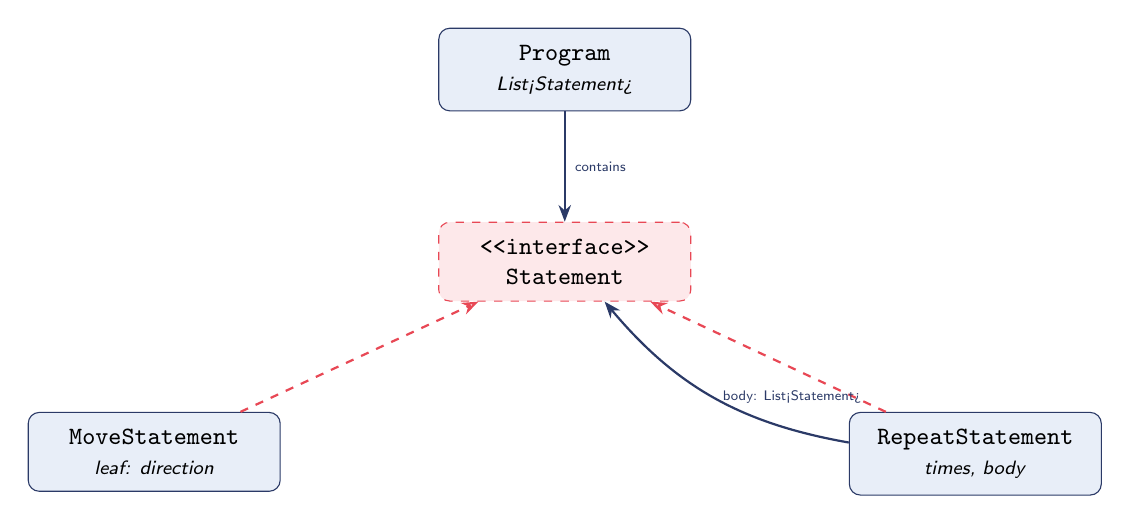
\begin{tikzpicture}[
  font=\sffamily\small,
  box/.style={rectangle, rounded corners=4pt, draw=primary, fill=sectionbg,
              minimum width=3.2cm, minimum height=0.8cm, inner sep=6pt,
              align=center},
  interface/.style={rectangle, rounded corners=4pt, draw=accent, fill=accentlight,
                    minimum width=3.2cm, minimum height=0.8cm, inner sep=6pt,
                    dashed, align=center},
  arr/.style={-{Stealth[length=6pt]}, primary, thick},
  impl/.style={-{Stealth[length=6pt, open]}, accent, thick, dashed},
  node distance=1.5cm and 2.5cm
]
  \node[interface] (stmt)  {\texttt{<<interface>>}\\ \texttt{Statement}};
  \node[box, below left=1.4cm and 2cm of stmt]  (move)   {\texttt{MoveStatement}\\ \scriptsize\textit{leaf: direction}};
  \node[box, below right=1.4cm and 2cm of stmt] (rep)    {\texttt{RepeatStatement}\\ \scriptsize\textit{times, body}};
  \node[box, above=1.4cm of stmt]               (prog)   {\texttt{Program}\\ \scriptsize\textit{List<Statement>}};

  \draw[impl] (move) -- (stmt);
  \draw[impl] (rep)  -- (stmt);
  \draw[arr]  (prog) -- (stmt) node[midway, right, font=\tiny\sffamily] {contains};
  \draw[arr, bend left=20]  (rep) to node[right, font=\tiny\sffamily]{body: List<Statement>} (stmt);
\end{tikzpicture}
\end{center}

\begin{tcolorbox}[gddbox, title={AST Node Descriptions}]
\begin{tabularx}{\linewidth}{>{\ttfamily\bfseries\color{primary}}p{3.5cm} X}
  \toprule
  \textrm{Node} & Fields \& Role \\
  \midrule
  \texttt{Program} & Root node. Contains an \texttt{unmodifiable List<Statement>}. Produced by \texttt{Parser.parse()} and consumed by \texttt{Interpreter.load()}. \\[4pt]
  \texttt{Statement} & Marker interface (no fields). Allows heterogeneous lists of statements. \\[4pt]
  \texttt{MoveStatement} & \texttt{Direction direction} (enum: UP, DOWN, LEFT, RIGHT). Leaf node — carries the direction the robot physically moves. \\[4pt]
  \texttt{RepeatStatement} & \texttt{int times} (validated 1--100); \texttt{List<Statement> body} (unmodifiable). Compound node — its body may contain further \texttt{RepeatStatement} nodes, enabling nesting. \\
  \bottomrule
\end{tabularx}
\end{tcolorbox}

\subsection{Sample Programs with Parse Trees}

\subsubsection{Example 1 — Simple path}

\begin{tcolorbox}[codebox, title={Robot Script Source}]
\begin{lstlisting}[language=RobotScript]
moveRight
moveRight
moveDown
moveRight
\end{lstlisting}
\end{tcolorbox}

\begin{center}
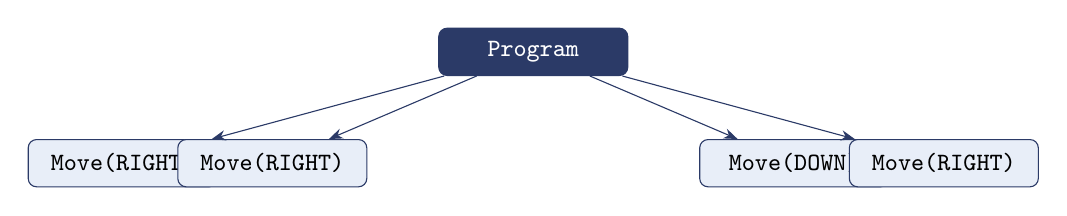
\begin{tikzpicture}[
  font=\sffamily\small,
  box/.style={rectangle, rounded corners=3pt, draw=primary, fill=sectionbg,
              minimum width=2.4cm, minimum height=0.6cm, inner sep=3pt},
  root/.style={rectangle, rounded corners=3pt, draw=primary, fill=primary,
               text=white, minimum width=2.4cm, minimum height=0.6cm, inner sep=3pt},
  arr/.style={-{Stealth[length=5pt]}, primary},
  node distance=1.0cm and 0.6cm
]
  \node[root] (p) {\texttt{Program}};
  \node[box, below left=0.8cm and 2.8cm of p]  (m1) {\texttt{Move(RIGHT)}};
  \node[box, below left=0.8cm and 0.9cm of p]  (m2) {\texttt{Move(RIGHT)}};
  \node[box, below right=0.8cm and 0.9cm of p] (m3) {\texttt{Move(DOWN)}};
  \node[box, below right=0.8cm and 2.8cm of p] (m4) {\texttt{Move(RIGHT)}};
  \draw[arr] (p) -- (m1);
  \draw[arr] (p) -- (m2);
  \draw[arr] (p) -- (m3);
  \draw[arr] (p) -- (m4);
\end{tikzpicture}
\end{center}

\subsubsection{Example 2 — Loop with nested repeat}

\begin{tcolorbox}[codebox, title={Robot Script Source — Nested Loop}]
\begin{lstlisting}[language=RobotScript]
repeat(3)
  moveRight
  repeat(2)
    moveDown
  end
end
moveUp
\end{lstlisting}
\end{tcolorbox}

\begin{center}
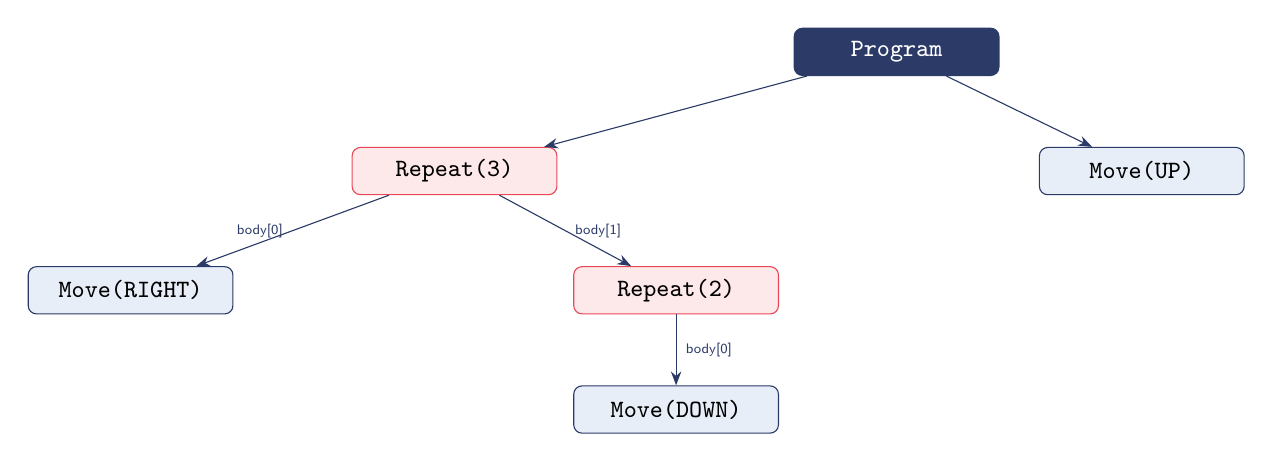
\begin{tikzpicture}[
  font=\sffamily\small,
  box/.style={rectangle, rounded corners=3pt, draw=primary, fill=sectionbg,
              minimum width=2.6cm, minimum height=0.6cm, inner sep=3pt},
  root/.style={rectangle, rounded corners=3pt, draw=primary, fill=primary,
               text=white, minimum width=2.6cm, minimum height=0.6cm, inner sep=3pt},
  loop/.style={rectangle, rounded corners=3pt, draw=accent, fill=accentlight,
               minimum width=2.6cm, minimum height=0.6cm, inner sep=3pt},
  arr/.style={-{Stealth[length=5pt]}, primary},
  labl/.style={font=\tiny\sffamily\color{accent}},
  node distance=1.0cm and 0.4cm
]
  \node[root] (p) {\texttt{Program}};
  \node[loop, below left=0.9cm and 3cm of p]  (r1) {\texttt{Repeat(3)}};
  \node[box,  below right=0.9cm and 0.5cm of p] (mu) {\texttt{Move(UP)}};

  \node[box,  below left=0.9cm and 1.5cm of r1] (mr) {\texttt{Move(RIGHT)}};
  \node[loop, below right=0.9cm and 0.2cm of r1] (r2) {\texttt{Repeat(2)}};

  \node[box,  below=0.9cm of r2] (md) {\texttt{Move(DOWN)}};

  \draw[arr] (p) -- (r1);
  \draw[arr] (p) -- (mu);
  \draw[arr] (r1) -- (mr) node[labl, midway, left] {body[0]};
  \draw[arr] (r1) -- (r2) node[labl, midway, right] {body[1]};
  \draw[arr] (r2) -- (md) node[labl, midway, right] {body[0]};
\end{tikzpicture}
\end{center}

The outer \texttt{Repeat(3)} executes its body 3 times. Each iteration: RIVETS moves right once, then down twice (inner loop). Total moves: 3 right + 6 down + 1 up.

\subsection{Execution Trace}

\begin{tcolorbox}[gddbox, title={Terminal Output — Example 2}]
\begin{lstlisting}[basicstyle=\ttfamily\small\color{codefg}, backgroundcolor=\color{codebg}, numbers=none]
~ # Running...
~ # moveRight
~ # moveDown
~ # moveDown
~ # moveRight
~ # moveDown
~ # moveDown
~ # moveRight
~ # moveDown
~ # moveDown
~ # moveUp
~ # Done in 1523 ms
\end{lstlisting}
\end{tcolorbox}

% ============================================================
\section{Technical Architecture}
% ============================================================

\subsection{Technology Stack}

\begin{tcolorbox}[gddbox, title={Technology Stack}]
\begin{tabularx}{\linewidth}{>{\bfseries\sffamily\color{primary}}p{4cm} X}
  \toprule
  Component & Details \\
  \midrule
  \textbf{Language}      & Java 11+ (compiled and run through the Greenfoot IDE) \\
  \textbf{Framework}     & Greenfoot 3.x — an educational 2D game framework built on top of Java 2D. Provides \texttt{World}, \texttt{Actor}, \texttt{GreenfootImage}, event loop, and key input. \\
  \textbf{Build system}  & Greenfoot project file (\texttt{.greenfoot}); standard \texttt{javac} compilation inside the IDE. \\
  \textbf{Version control} & Git (GitHub repository: \texttt{codebot-maze-serious-game}) \\
  \textbf{Target platform} & Desktop (Windows, macOS, Linux) running Greenfoot 3.x / JDK 11+ \\
  \bottomrule
\end{tabularx}
\end{tcolorbox}

\subsection{System Architecture Overview}

The system is organised into five distinct subsystems, each with clear responsibilities and minimal coupling.

\begin{center}
\begin{tikzpicture}[
  font=\sffamily\small,
  subsys/.style={rectangle, rounded corners=6pt, draw=primary, fill=sectionbg,
                 minimum width=3.5cm, minimum height=1.2cm, inner sep=8pt,
                 align=center},
  arr/.style={-{Stealth[length=7pt]}, primary!70, thick},
  labl/.style={font=\scriptsize\sffamily, fill=white, inner sep=2pt},
  node distance=1.4cm and 0.5cm
]
  \node[subsys, fill=primary!15] (ui) {\textbf{UI Layer}\\ {\scriptsize HomeWorld, MyWorld,\\ CodeEditor, MenuButton}};

  \node[subsys, fill=accent!10, right=3.5cm of ui] (lex) {\textbf{Lexer}\\ {\scriptsize Tokenises source text\\ \(\rightarrow\) List<Token>}};
  \node[subsys, fill=accent!10, right=3.5cm of lex] (par) {\textbf{Parser}\\ {\scriptsize Recursive descent\\ \(\rightarrow\) Program (AST)}};

  \node[subsys, fill=primary!20, below=2cm of par] (interp) {\textbf{Interpreter}\\ {\scriptsize Stack-based execution\\ next() per act() frame}};
  \node[subsys, fill=primary!15, below=2cm of ui]  (robot) {\textbf{RobotActor}\\ {\scriptsize Movement, collision,\\ goal detection}};

  \node[subsys, fill=gridbg, below=2cm of lex] (level) {\textbf{Level System}\\ {\scriptsize Level interface\\ Level1, LevelManager}};

  \draw[arr] (ui)     -- node[labl, above]{source text} (lex);
  \draw[arr] (lex)    -- node[labl, above]{tokens}      (par);
  \draw[arr] (par)    -- node[labl, right]{Program}     (interp);
  \draw[arr] (interp) -- node[labl, above]{MoveStatement} (robot);
  \draw[arr] (ui)     -- node[labl, left]{RUN / RESET}  (robot);
  \draw[arr] (level)  -- node[labl, below]{setup()}     (ui);
\end{tikzpicture}
\end{center}

\subsection{Execution Pipeline}

\begin{center}
\begin{tikzpicture}[
  font=\sffamily\small,
  step/.style={rectangle, rounded corners=5pt, draw=primary, fill=sectionbg,
               minimum width=3cm, minimum height=1.1cm, inner sep=6pt},
  data/.style={rectangle, rounded corners=3pt, draw=accent!70, fill=accentlight,
               minimum width=2.4cm, minimum height=0.7cm, inner sep=4pt,
               font=\ttfamily\scriptsize},
  arr/.style={-{Stealth[length=6pt]}, primary, thick},
  node distance=0.8cm and 0.2cm
]
  \node[step] (src)   {\textbf{1. Source Text}\\{\scriptsize Player's typed code}};
  \node[data, right=0.4cm of src] (tok) {List<Token>};
  \node[step, right=0.4cm of tok] (lex) {\textbf{2. Lexer}\\{\scriptsize \texttt{Lexer.tokenize()}}};
  \node[data, right=0.4cm of lex] (ast) {Program (AST)};
  \node[step, right=0.4cm of ast] (par) {\textbf{3. Parser}\\{\scriptsize \texttt{Parser.parse()}}};

  \node[step, below=1.2cm of par] (itp) {\textbf{4. Interpreter}\\{\scriptsize \texttt{.load(program)}}};
  \node[data, left=0.4cm of itp] (mv) {MoveStatement};
  \node[step, left=0.4cm of mv]  (rob) {\textbf{5. RobotActor}\\{\scriptsize \texttt{.executeMove()}}};
  \node[step, left=0.4cm of rob] (anim) {\textbf{6. Animation}\\{\scriptsize Greenfoot act() loop}};

  \draw[arr] (src)  -- (tok);
  \draw[arr] (tok)  -- (lex);
  \draw[arr] (lex)  -- (ast);
  \draw[arr] (ast)  -- (par);
  \draw[arr] (par)  -- (itp);
  \draw[arr] (itp)  -- (mv);
  \draw[arr] (mv)   -- (rob);
  \draw[arr] (rob)  -- (anim);
\end{tikzpicture}
\end{center}

\vspace{6pt}
\textbf{Key insight — frame-by-frame execution:} Greenfoot's game loop calls \texttt{act()} once per frame on every actor. \texttt{RobotActor.act()} calls \texttt{interpreter.next()}, which returns exactly one \texttt{MoveStatement} per call. This couples one animation frame to one logical instruction — the player sees the robot move step-by-step rather than teleporting to the end position. The Interpreter uses an \textbf{explicit stack of Frames} instead of Java recursion, because recursive traversal of the AST would complete the entire program in a single frame with no animation.

\subsection{Class Diagram}

\begin{center}
\scriptsize
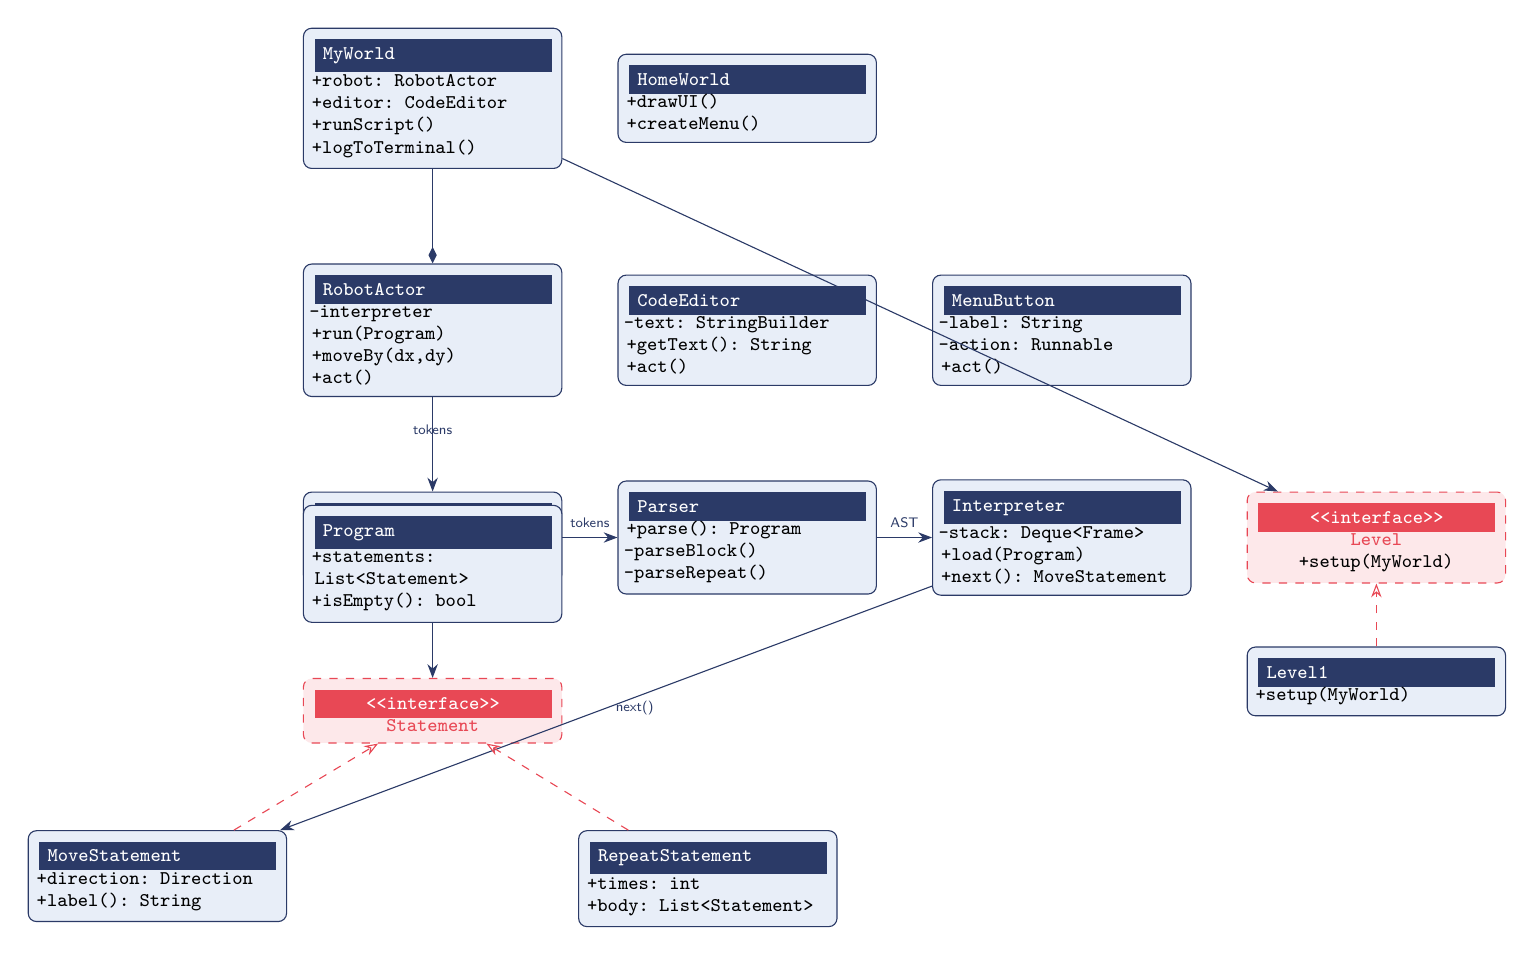
\begin{tikzpicture}[
  font=\sffamily\scriptsize,
  cls/.style={rectangle, draw=primary, fill=sectionbg, rounded corners=3pt,
              inner sep=4pt, align=left, text width=3.0cm},
  iface/.style={rectangle, draw=accent, fill=accentlight, dashed, rounded corners=3pt,
                inner sep=4pt, align=center, text width=3.0cm},
  arr/.style={-{Stealth[length=5pt]}, primary},
  impl/.style={-{Stealth[length=5pt, open]}, accent, dashed},
  comp/.style={-{Diamond[length=6pt]}, primary},
  node distance=1.6cm and 0.6cm
]
  % ── Row 1: Worlds ──────────────────────────────────────────────────────────
  \node[cls] (mw) {%
    \textcolor{white}{\colorbox{primary}{\makebox[2.8cm][l]{\textbf{\texttt{MyWorld}}}}}\par
    \texttt{+robot: RobotActor}\par
    \texttt{+editor: CodeEditor}\par
    \texttt{+runScript()}\par
    \texttt{+logToTerminal()}};

  \node[cls, right=0.7cm of mw] (hw) {%
    \textcolor{white}{\colorbox{primary}{\makebox[2.8cm][l]{\textbf{\texttt{HomeWorld}}}}}\par
    \texttt{+drawUI()}\par
    \texttt{+createMenu()}};

  % ── Row 2: Actors ──────────────────────────────────────────────────────────
  \node[cls, below=1.2cm of mw] (ra) {%
    \textcolor{white}{\colorbox{primary}{\makebox[2.8cm][l]{\textbf{\texttt{RobotActor}}}}}\par
    \texttt{-interpreter}\par
    \texttt{+run(Program)}\par
    \texttt{+moveBy(dx,dy)}\par
    \texttt{+act()}};

  \node[cls, right=0.7cm of ra] (ce) {%
    \textcolor{white}{\colorbox{primary}{\makebox[2.8cm][l]{\textbf{\texttt{CodeEditor}}}}}\par
    \texttt{-text: StringBuilder}\par
    \texttt{+getText(): String}\par
    \texttt{+act()}};

  \node[cls, right=0.7cm of ce] (mb) {%
    \textcolor{white}{\colorbox{primary}{\makebox[2.8cm][l]{\textbf{\texttt{MenuButton}}}}}\par
    \texttt{-label: String}\par
    \texttt{-action: Runnable}\par
    \texttt{+act()}};

  % ── Row 3: DSL pipeline ─────────────────────────────────────────────────────
  \node[cls, below=1.2cm of ra] (lx) {%
    \textcolor{white}{\colorbox{primary}{\makebox[2.8cm][l]{\textbf{\texttt{Lexer}}}}}\par
    \texttt{+tokenize()}\par
    \texttt{+keywordType(...)}};

  \node[cls, right=0.7cm of lx] (px) {%
    \textcolor{white}{\colorbox{primary}{\makebox[2.8cm][l]{\textbf{\texttt{Parser}}}}}\par
    \texttt{+parse(): Program}\par
    \texttt{-parseBlock()}\par
    \texttt{-parseRepeat()}};

  \node[cls, right=0.7cm of px] (ix) {%
    \textcolor{white}{\colorbox{primary}{\makebox[2.8cm][l]{\textbf{\texttt{Interpreter}}}}}\par
    \texttt{-stack: Deque<Frame>}\par
    \texttt{+load(Program)}\par
    \texttt{+next(): MoveStatement}};

  % ── Row 4: AST ──────────────────────────────────────────────────────────────
  \node[iface, below=1.2cm of lx] (st) {%
    \textcolor{white}{\colorbox{accent}{\makebox[2.8cm][c]{\textbf{\texttt{<<interface>>}}}}}\par
    \textcolor{accent}{\textbf{\texttt{Statement}}}};

  \node[cls, below left=1.1cm and 0.2cm of st] (ms) {%
    \textcolor{white}{\colorbox{primary}{\makebox[2.8cm][l]{\textbf{\texttt{MoveStatement}}}}}\par
    \texttt{+direction: Direction}\par
    \texttt{+label(): String}};

  \node[cls, below right=1.1cm and 0.2cm of st] (rs) {%
    \textcolor{white}{\colorbox{primary}{\makebox[2.8cm][l]{\textbf{\texttt{RepeatStatement}}}}}\par
    \texttt{+times: int}\par
    \texttt{+body: List<Statement>}};

  \node[cls, above=0.7cm of st] (pg) {%
    \textcolor{white}{\colorbox{primary}{\makebox[2.8cm][l]{\textbf{\texttt{Program}}}}}\par
    \texttt{+statements: List<Statement>}\par
    \texttt{+isEmpty(): bool}};

  % ── Level interface ─────────────────────────────────────────────────────────
  \node[iface, right=0.7cm of ix] (lvl) {%
    \textcolor{white}{\colorbox{accent}{\makebox[2.8cm][c]{\textbf{\texttt{<<interface>>}}}}}\par
    \textcolor{accent}{\textbf{\texttt{Level}}}\par
    \texttt{+setup(MyWorld)}};

  \node[cls, below=0.8cm of lvl] (l1) {%
    \textcolor{white}{\colorbox{primary}{\makebox[2.8cm][l]{\textbf{\texttt{Level1}}}}}\par
    \texttt{+setup(MyWorld)}};

  % ── Arrows ──────────────────────────────────────────────────────────────────
  \draw[comp] (mw.south) -- (ra.north);
  \draw[arr]  (ra) -- node[above,font=\tiny\sffamily]{tokens} (lx);
  \draw[arr]  (lx) -- node[above,font=\tiny\sffamily]{tokens} (px);
  \draw[arr]  (px) -- node[above,font=\tiny\sffamily]{AST} (ix);
  \draw[arr]  (ix) -- node[right,font=\tiny\sffamily]{next()} (ms);
  \draw[arr]  (pg) -- (st);
  \draw[impl] (ms) -- (st);
  \draw[impl] (rs) -- (st);
  \draw[impl] (l1) -- (lvl);
  \draw[arr]  (mw) -- (lvl);
\end{tikzpicture}
\end{center}

\subsection{Interpreter Stack-Frame Model}

The Interpreter maintains a \texttt{Deque<Frame>} where each \texttt{Frame} tracks:

\begin{itemize}[noitemsep]
  \item \texttt{stmts}: the list of statements in this block
  \item \texttt{index}: which statement to execute next
  \item \texttt{iteration}: current loop pass (0-based)
  \item \texttt{totalIter}: total loop iterations (always 1 for top-level)
\end{itemize}

\begin{tcolorbox}[gddbox, title={Frame Lifecycle}]
\begin{tabularx}{\linewidth}{>{\bfseries\sffamily\color{primary}}p{3.5cm} X}
  \toprule
  Event & Action \\
  \midrule
  \texttt{load(program)} & Push one top-level Frame with \texttt{totalIter=1}. \\
  \texttt{MoveStatement} encountered & Return it to \texttt{RobotActor}; advance \texttt{index}. \\
  \texttt{RepeatStatement} encountered & Push new Frame with \texttt{totalIter=repeat.times}. \\
  \texttt{index >= stmts.size()} (block exhausted) & Increment \texttt{iteration}. If \texttt{iteration < totalIter}: reset \texttt{index=0} (next loop pass). Else: pop Frame. \\
  Stack empty & Set \texttt{running=false}; return \texttt{null}. \\
  \bottomrule
\end{tabularx}
\end{tcolorbox}

\subsection{Error Handling Pipeline}

\begin{tcolorbox}[redbox, title={Error Types and User Feedback}]
\begin{tabularx}{\linewidth}{>{\bfseries\sffamily\color{accent}}p{3cm} >{\ttfamily\scriptsize}p{4cm} X}
  \toprule
  \textrm{Error type} & Exception class & Terminal message \\
  \midrule
  Unknown character & \texttt{Lexer.LexError} & \texttt{[LEX ERROR] Line N: Unexpected character: 'X'} \\
  Unknown keyword   & \texttt{Lexer.LexError} & \texttt{[LEX ERROR] Line N: Unknown keyword: 'foo'} \\
  Missing \texttt{()} after repeat & \texttt{Parser.ParseError} & \texttt{[PARSE ERROR] Line N: Expected LPAREN but got 'X'} \\
  Loop count out of range & \texttt{Parser.ParseError} & \texttt{[PARSE ERROR] Line N: repeat count must be between 1 and 100} \\
  Missing \texttt{end} keyword & \texttt{Parser.ParseError} & \texttt{[PARSE ERROR] Line N: Expected 'end' to close repeat(N)} \\
  Empty program & \textit{(no exception)} & \texttt{[!] Program is empty} \\
  Robot blocked & \textit{(no exception)} & \texttt{[!] Blocked by obstacle} \\
  \bottomrule
\end{tabularx}
\end{tcolorbox}

% ============================================================
\section{Level Design}
% ============================================================

\subsection{Level Design Principles}

\begin{tcolorbox}[gddbox, title={Level Design Philosophy}]
\begin{enumerate}[label=\textbf{P\arabic*.}, leftmargin=3em, noitemsep]
  \item \textbf{Introduce one concept per level.} Level 1 introduces movement only. Subsequent levels introduce obstacles, then loops, then nested loops.
  \item \textbf{Solvable without loops first.} Every level can be completed with only move commands. Loops are rewarded (fewer instructions) but never required.
  \item \textbf{Visual clarity.} The optimal path is visible by inspection. Players should be able to trace the route with their eyes before coding.
  \item \textbf{Grid alignment.} All objects are placed on 20-pixel grid boundaries. Start and goal positions are chosen so that integer arithmetic always gives the correct move count.
\end{enumerate}
\end{tcolorbox}

\subsection{Level 1 — Tutorial}

\begin{tcolorbox}[gddbox, title={Level 1 Specification}]
\gddfield{Robot start:}{\texttt{(100, 100)} — top-left quadrant of the game area}
\gddfield{Goal position:}{\texttt{(500, 300)} — centre-right}
\gddfield{Obstacles:}{\texttt{(300, 200)}, \texttt{(300, 220)}, \texttt{(300, 240)} — a vertical wall of 3 blocks}
\gddfield{Optimal solution:}{Move right 10 times, down 8 times (going around the wall); or \texttt{repeat(10)\{moveRight\}end} + \texttt{repeat(8)\{moveDown\}end}}
\gddfield{Learning goal:}{Practice basic movement; observe what happens when the robot walks into a wall.}
\end{tcolorbox}

\begin{center}
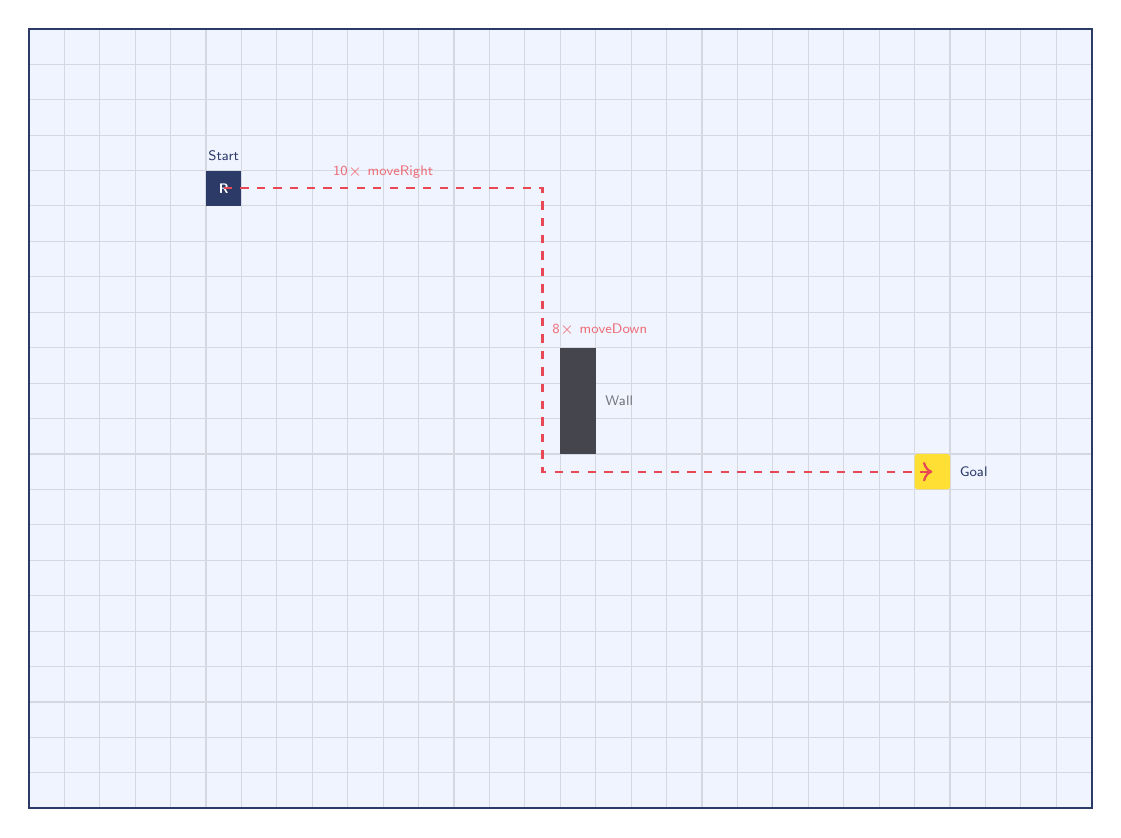
\begin{tikzpicture}[font=\sffamily\tiny, scale=0.45]
  % Grid
  \fill[gridbg] (0,0) rectangle (30,22);
  \draw[primary!20, step=1] (0,0) grid (30,22);
  \draw[primary, thick] (0,0) rectangle (30,22);
  % Robot start (5,5 in grid units: 100/20=5, 100/20=5)
  \fill[primary] (5,17) rectangle (6,18);
  \node[white, font=\bfseries\sffamily\tiny] at (5.5,17.5) {R};
  % Goal (25,15 in grid: 500/20=25, but grid Y is inverted: (600-300)/20=15)
  \fill[number!80, rounded corners=1pt] (25,9) rectangle (26,10);
  \node[font=\bfseries\sffamily\tiny, number!80] at (25.5,9.5) {$\star$};
  % Obstacles (300/20=15, 200/20=10 → inverted: 22-10=12)
  \fill[darkbg!80] (15,12) rectangle (16,13);
  \fill[darkbg!80] (15,11) rectangle (16,12);
  \fill[darkbg!80] (15,10) rectangle (16,11);
  % Path arrow (simplified)
  \draw[->, accent, thick, dashed] (5.5,17.5) -- (14.5,17.5) -- (14.5,9.5) -- (25.5,9.5);
  % Labels
  \node[primary, above] at (5.5,18) {Start};
  \node[primary, right] at (26,9.5) {Goal};
  \node[darkbg!60, right] at (16,11.5) {Wall};
  \node[accent!80, above] at (10,17.5) {\tiny 10$\times$ moveRight};
  \node[accent!80, right] at (14.5,13.5) {\tiny 8$\times$ moveDown};
\end{tikzpicture}
\end{center}

\subsection{Level Progression Plan}

\begin{center}
\begin{tabularx}{\linewidth}{>{\bfseries\sffamily\color{primary}}c >{\bfseries\sffamily}p{3cm} X >{\sffamily}p{3cm}}
  \toprule
  Level & Name & New Concept & Key Mechanic Taught \\
  \midrule
  1 & Tutorial Path & Basic movement; single vertical wall & Sequential instructions \\
  2 & L-Turn Maze & Corner turns with multiple walls & Planning compound paths \\
  3 & Long Corridor & Long repeated movement & Using \keyword{repeat} for efficiency \\
  4 & Zigzag Alley & Alternating direction pattern & Recognising repeating sub-paths \\
  5 & Nested Chambers & Inner loops within outer loops & Nested \keyword{repeat} \\
  6 & The Labyrinth & Dense obstacle field; multiple valid paths & Algorithm design and debugging \\
  \bottomrule
\end{tabularx}
\end{center}

% ============================================================
\section{Technical Requirements}
% ============================================================

\subsection{Platform}

\begin{tcolorbox}[gddbox, title={Platform}]
\gddfield{Target environment:}{Desktop operating systems: \textbf{Windows 10/11}, \textbf{macOS 12+}, \textbf{Ubuntu 20.04+}}
\gddfield{Runtime:}{Java Runtime Environment (JRE) 11 or higher, bundled with Greenfoot 3.x installer.}
\gddfield{Distribution:}{Greenfoot project folder (source + compiled \texttt{.class} files), run inside Greenfoot IDE. Optionally exportable as a standalone \texttt{.jar} using Greenfoot's built-in export feature.}
\end{tcolorbox}

\subsection{Development Environment}

\begin{tcolorbox}[gddbox, title={Development Environment}]
\begin{tabularx}{\linewidth}{>{\bfseries\sffamily\color{primary}}p{4cm} X}
  \toprule
  Tool & Role \\
  \midrule
  \textbf{Greenfoot 3.7+}    & Primary IDE and game framework; built-in Java compiler and runner \\
  \textbf{JDK 11+}           & Java compiler (\texttt{javac}) and runtime (\texttt{java}) \\
  \textbf{Git + GitHub}      & Version control and collaboration (\texttt{codebot-maze-serious-game} repository) \\
  \textbf{VS Code}           & Secondary editor for larger refactoring tasks \\
  \textbf{IntelliJ IDEA}     & Optional; used for static analysis and refactoring \\
  \textbf{draw.io / Miro}    & Architecture and level design diagrams \\
  \bottomrule
\end{tabularx}
\end{tcolorbox}

\subsection{System Requirements}

\begin{tcolorbox}[gddbox, title={End-User System Requirements}]
\begin{tabularx}{\linewidth}{>{\bfseries\sffamily\color{primary}}p{4cm} X}
  \toprule
  Requirement & Minimum Specification \\
  \midrule
  \textbf{OS}           & Windows 10, macOS 12, Ubuntu 20.04 (or newer) \\
  \textbf{Java}         & JRE 11+ (included in Greenfoot installer) \\
  \textbf{RAM}          & 512 MB available (Greenfoot + JVM) \\
  \textbf{Disk}         & 250 MB (Greenfoot installation) + $<$10 MB (game project) \\
  \textbf{Display}      & Minimum 1024$\times$768 (game window is 800$\times$600) \\
  \textbf{Input}        & Standard keyboard (mouse optional for buttons) \\
  \textbf{Network}      & None required (fully offline) \\
  \bottomrule
\end{tabularx}
\end{tcolorbox}

\subsection{Resourcing and Capability}

\begin{tcolorbox}[gddbox, title={Resourcing / Capability}]
\begin{tabularx}{\linewidth}{>{\bfseries\sffamily\color{primary}}p{4cm} X}
  \toprule
  Area & Details \\
  \midrule
  \textbf{Core skills required} & Java OOP; Greenfoot Actor/World API; basic compiler theory (Lexer/Parser patterns); 2D game design \\
  \textbf{Graphics tools} & Greenfoot built-in \texttt{GreenfootImage} drawing API (programmatic); optionally GIMP or Aseprite for sprite creation \\
  \textbf{Audio tools} & Greenfoot's \texttt{GreenfootSound} API for simple SFX (future iteration) \\
  \textbf{Testing} & Manual playtesting; JUnit 5 for Lexer and Parser unit tests \\
  \textbf{Responsibilities} & \emph{Team Captain}: architecture, Lexer/Parser/Interpreter; \emph{Member 2}: Greenfoot worlds, UI; \emph{Member 3}: level design, graphics; \emph{Member 4}: testing, documentation \\
  \bottomrule
\end{tabularx}
\end{tcolorbox}

% ============================================================
\section{Visuals, Artwork, and Graphics}
% ============================================================

\subsection{Visual Style}

\begin{tcolorbox}[gddbox, title={Visual Style}]
\gddfield{Overall aesthetic:}{\textbf{Minimalist dark-theme} — inspired by modern code editors (VS Code dark, Monokai). The dark background reduces eye strain during long play sessions and makes the bright robot and goal objects ``pop'' visually.}

\vspace{4pt}
\begin{tabularx}{\linewidth}{>{\bfseries\sffamily\color{primary}}p{3.5cm} X}
  \toprule
  Element & Colour / Style \\
  \midrule
  Game area background & Light grey (\texttt{\#D3D3D3}) — neutral, grid-scannable \\
  Code editor bg & Deep navy-black (\texttt{\#16161F}) — code editor aesthetic \\
  Terminal bg & Near-black (\texttt{\#161616}) \\
  Terminal text & Soft green (\texttt{\#B4F0B4}) — classic terminal green \\
  Keyword highlight & Cornflower blue (\texttt{\#7FAAFF}) — standard syntax colour \\
  Number highlight & Gold (\texttt{\#FFD700}) \\
  RIVETS (robot) & Primary blue body, red accent eyes — friendly, mechanical \\
  Goal tile & Glowing gold / yellow star \\
  Obstacle & Dark charcoal block — visually solid and impenetrable \\
  UI controls bg & Dark blue-grey (\texttt{\#232337}) \\
  Editor border & Periwinkle (\texttt{\#4646A0}) \\
  \bottomrule
\end{tabularx}

\vspace{6pt}
\gddfield{Character style:}{RIVETS is rendered programmatically using \texttt{GreenfootImage} shape-drawing calls — rectangles, circles, and filled arcs — giving a clean vector-like appearance that scales well and requires no external sprite assets.}
\gddfield{Font:}{\texttt{Monospaced} for code editor and terminal; \texttt{Font(11)} or \texttt{Font(12)} for all other UI text. Consistent monospacing reinforces the ``code is text'' paradigm.}
\end{tcolorbox}

\subsection{Colour Palette Reference}

\begin{center}
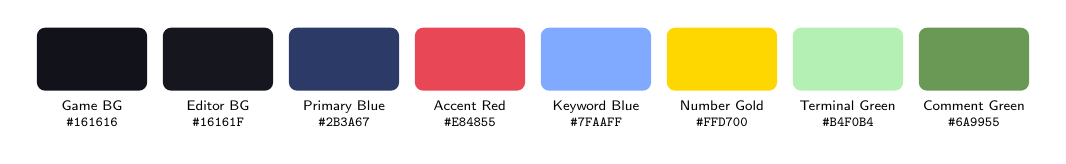
\begin{tikzpicture}[font=\sffamily\tiny]
  \foreach \col/\name/\hex/\i in {
    darkbg!80!black/Game BG/161616/0,
    codebg/Editor BG/16161F/1,
    primary/Primary Blue/2B3A67/2,
    accent/Accent Red/E84855/3,
    keyword/Keyword Blue/7FAAFF/4,
    number/Number Gold/FFD700/5,
    codefg/Terminal Green/B4F0B4/6,
    comment/Comment Green/6A9955/7
  } {
    \fill[\col, rounded corners=3pt] (\i*1.6, 0) rectangle (\i*1.6+1.4, 0.8);
    \node[below, text width=1.4cm, align=center] at (\i*1.6+0.7, 0) {\name\\\texttt{\#\hex}};
  }
\end{tikzpicture}
\end{center}

\subsection{Art Production Process}

\begin{tcolorbox}[gddbox, title={Art Process}]
\gddfield{Concept stage:}{Sketch UI layout and robot character on paper / draw.io. Define colour palette. Agree on grid cell size (20 px) and window resolution (800$\times$600).}
\gddfield{Implementation:}{All game visuals are rendered via Greenfoot's \texttt{GreenfootImage} Java API. This ``code-drawn'' approach means:
\begin{itemize}[noitemsep]
  \item No external image files needed (except the logo/splash).
  \item Colours and sizes are constants in source code — trivially adjustable.
  \item Retina / HiDPI screens: Greenfoot handles Java2D rendering; resolution-independent to the extent the JVM supports.
\end{itemize}
}
\gddfield{Syntax highlighting:}{\texttt{CodeSyntaxHighlighter} uses the \texttt{Lexer.keywordTypeForLowercase()} method to colour-classify each word in the editor as the player types. This keeps keyword definitions in a single place and makes the highlighter automatically correct when new keywords are added.}
\gddfield{Future assets:}{If time permits: (a) Aseprite sprite sheet for RIVETS with walk animation frames; (b) particle effect on goal collision; (c) background tileset for themed level environments (factory, space, underwater).}
\end{tcolorbox}

% ============================================================
\section{Timeline and Project Planning}
% ============================================================

\subsection{Deadline}

\begin{tcolorbox}[redbox, title={Submission Deadline}]
\gddfield{Final submission:}{\textbf{[Insert challenge deadline date]}}
\gddfield{Internal code freeze:}{One week before submission — no new features after this date; bug fixes only.}
\gddfield{Playtest deadline:}{Two weeks before submission — at least three external playtesters must have completed Level 1--3.}
\end{tcolorbox}

\subsection{Development Timeline}

\begin{center}
\begin{tikzpicture}[font=\sffamily\small, x=1.45cm, y=0.85cm]
  % Swimlane headers
  \foreach \lane/\label/\col in {
    0/Architecture \& DSL/primary,
    1/Gameplay \& Levels/primary!70,
    2/UI \& Graphics/accent,
    3/Testing \& Docs/primary!50
  } {
    \fill[\col!20] (-0.1, -\lane-0.45) rectangle (0.9, -\lane+0.45);
    \node[font=\sffamily\tiny\bfseries, \col, align=left, text width=1.8cm]
      at (0.4, -\lane) {\label};
  }
  % Week bars
  \foreach \week in {1,...,8} {
    \draw[primary!20, thin] (\week+0.8, 0.6) -- (\week+0.8, -3.6);
    \node[primary!60, font=\tiny\sffamily] at (\week+1.3, 0.8) {Wk\week};
  }
  % Tasks
  % Architecture & DSL
  \fill[primary!70, rounded corners=2pt] (1.9,-0.3) rectangle (4.7,0.3);
  \node[white, font=\tiny\sffamily] at (3.3, 0) {Lexer + Parser + Interpreter};
  \fill[primary!40, rounded corners=2pt] (4.9,-0.3) rectangle (6.7,0.3);
  \node[white, font=\tiny\sffamily] at (5.8, 0) {Refine \& unit test};
  % Gameplay & Levels
  \fill[primary!60, rounded corners=2pt] (1.9,-1.3) rectangle (3.7,-0.7);
  \node[white, font=\tiny\sffamily] at (2.8, -1) {World layout};
  \fill[primary!50, rounded corners=2pt] (3.9,-1.3) rectangle (6.7,-0.7);
  \node[white, font=\tiny\sffamily] at (5.3, -1) {Level 1--6 design \& build};
  \fill[primary!30, rounded corners=2pt] (6.9,-1.3) rectangle (8.7,-0.7);
  \node[primary!80, font=\tiny\sffamily] at (7.8, -1) {Polish};
  % UI & Graphics
  \fill[accent!70, rounded corners=2pt] (1.9,-2.3) rectangle (4.7,-1.7);
  \node[white, font=\tiny\sffamily] at (3.3, -2) {CodeEditor + Terminal};
  \fill[accent!50, rounded corners=2pt] (4.9,-2.3) rectangle (7.7,-1.7);
  \node[white, font=\tiny\sffamily] at (6.3, -2) {RIVETS sprite, Menus, SFX};
  % Testing & Docs
  \fill[primary!40, rounded corners=2pt] (5.9,-3.3) rectangle (7.7,-2.7);
  \node[white, font=\tiny\sffamily] at (6.8, -3) {Playtesting};
  \fill[primary!25, rounded corners=2pt] (7.9,-3.3) rectangle (9.7,-2.7);
  \node[primary!70, font=\tiny\sffamily] at (8.8, -3) {GDD \& submission};
  % Code freeze line
  \draw[accent, thick, dashed] (8.9, 0.6) -- (8.9, -3.6);
  \node[accent, font=\tiny\bfseries, rotate=90] at (8.75,-1.5) {CODE FREEZE};
\end{tikzpicture}
\end{center}

\begin{tcolorbox}[gddbox, title={Milestone Summary}]
\begin{tabularx}{\linewidth}{>{\bfseries\sffamily\color{primary}}p{2.5cm} >{\bfseries}p{1.5cm} X}
  \toprule
  Milestone & Week & Deliverable \\
  \midrule
  M1 — DSL Core    & Week 2 & Lexer + Parser + Interpreter unit-tested; simple program runs in console \\
  M2 — Game Loop   & Week 3 & RobotActor animates in Greenfoot world; Level 1 playable \\
  M3 — Editor live & Week 4 & CodeEditor with syntax highlighting; RUN/RESET buttons work \\
  M4 — Levels 1--4 & Week 5 & Four playable levels with obstacles and loops \\
  M5 — Full game   & Week 7 & All 6 levels; Home screen; Instructions; Credits \\
  M6 — Submission  & Week 8 & GDD final; game exported; playtesting complete \\
  \bottomrule
\end{tabularx}
\end{tcolorbox}

% ============================================================
\section{Risk Assessment}
% ============================================================

\begin{tcolorbox}[gddbox, title={Risk Register}]
\begin{tabularx}{\linewidth}{>{\bfseries\sffamily\color{primary}}p{3.5cm} >{\centering}p{1.5cm} >{\centering}p{1.5cm} X}
  \toprule
  Risk & Likelihood & Impact & Mitigation \\
  \midrule
  Greenfoot act() loop too slow for smooth animation & Medium & High & Use \texttt{Greenfoot.delay()} tuning; profile on target machine early \\
  Keyboard input inconsistency across Greenfoot builds & High & Medium & Defensive coding in \texttt{CodeEditor} handles both known key-naming variants \\
  Scope creep (too many language features) & Medium & High & Hard language freeze at 6 keywords; extra features go in ``future work'' section \\
  Team member unavailability & Low & Medium & Git branching; any member can pick up any module from clear docs \\
  Parser/Interpreter bugs for deeply nested loops & Low & High & Unit test all nesting combinations up to depth 3 before integration \\
  Level design too hard for target age group & Medium & Medium & External playtests with 12--14 year-olds in Week 6; iterate on difficulty curve \\
  \bottomrule
\end{tabularx}
\end{tcolorbox}

% ============================================================
\section{Educational Outcomes}
% ============================================================

\begin{tcolorbox}[gddbox, title={Learning Outcomes Mapped to Core Curriculum}]
\begin{tabularx}{\linewidth}{>{\bfseries\sffamily\color{primary}}p{4cm} X}
  \toprule
  Learning focus & How Robot Programmer addresses it \\
  \midrule
  \textbf{Digital Technologies — Algorithms} & Players write explicit step-by-step algorithms (programs) that the robot executes exactly as written \\
  \textbf{Computational Thinking — Sequencing} & Every move command is a sequence element; order matters and is visible in the terminal output \\
  \textbf{Loops and Iteration} & The \keyword{repeat} construct directly teaches counted loops — the most common structure in beginner programming \\
  \textbf{Debugging} & Plain-English error messages on the terminal encourage read–fix–rerun cycles identical to real development \\
  \textbf{Abstraction} & Players think about paths and directions, not about pixels or JVM internals \\
  \textbf{Problem decomposition} & Complex maze routes are naturally decomposed into movement phases, each expressed as a block of code \\
  \bottomrule
\end{tabularx}
\end{tcolorbox}

% ============================================================
\section{Future Work and Extensions}
% ============================================================

\begin{tcolorbox}[gddbox, title={Planned Future Extensions (Post-submission)}]
\begin{enumerate}[label=\textbf{F\arabic*.}, leftmargin=3em]
  \item \textbf{Variables.} Add \keyword{set x 5} and \keyword{move x} syntax, introducing the concept of named values.
  \item \textbf{Conditionals.} Add \keyword{if wall} / \keyword{else} / \keyword{endif} so the robot can react to its environment — teaching branching logic.
  \item \textbf{Procedures.} Add \keyword{define} / \keyword{call} so players can name and reuse sub-programs — teaching functions and modularity.
  \item \textbf{Level editor.} A drag-and-place tool allowing teachers to design custom mazes and export them as \texttt{LevelN.java} files.
  \item \textbf{Multiplayer / competition mode.} Two robots on the same grid; both players submit programs; first to reach the goal wins.
  \item \textbf{Step-through debugger.} A ``STEP'' button that executes one instruction at a time, highlighting the corresponding line in the editor — reinforcing the connection between source code and machine state.
  \item \textbf{Analytics export.} Log anonymised attempt counts, error types, and solution lengths per level for classroom research.
\end{enumerate}
\end{tcolorbox}

% ============================================================
\section{Appendix A — Complete Grammar Reference}
% ============================================================

\begin{tcolorbox}[codebox, title={Robot Script — Complete Formal Specification}]
\begin{lstlisting}[style=ebnf]
(*  Robot Script DSL - Formal Grammar (ISO/IEC 14977 EBNF)  *)

program     = { statement } , EOF ;

statement   = move
            | repeat-stmt ;

move        = "moveUp"
            | "moveDown"
            | "moveLeft"
            | "moveRight" ;

repeat-stmt = "repeat" , "(" , number , ")" ,
                  { statement } ,
              "end" ;

number      = digit , { digit } ;
digit       = "0" | "1" | "2" | "3" | "4"
            | "5" | "6" | "7" | "8" | "9" ;

(*  Lexical notes:
    - All keywords are case-insensitive.
    - Whitespace (space, tab, newline) is ignored between tokens.
    - NUMBER is validated at parse-time to be in [1, 100].
    - Unrecognised characters raise LexError with line number.
    - Unrecognised keywords raise LexError with line number.
*)
\end{lstlisting}
\end{tcolorbox}

% ============================================================
\section{Appendix B — Key Source Code Excerpts}
% ============================================================

\subsection{Interpreter — Core next() Method}

\begin{tcolorbox}[codebox, title={Interpreter.java — next()}]
\begin{lstlisting}[style=java]
public MoveStatement next() {
    while (!stack.isEmpty()) {
        Frame frame = stack.peek();

        // Block exhausted?
        if (frame.index >= frame.stmts.size()) {
            frame.iteration++;
            if (frame.iteration < frame.totalIter) {
                frame.index = 0;   // next loop pass
            } else {
                stack.pop();       // loop finished
            }
            continue;
        }

        Statement stmt = frame.stmts.get(frame.index++);

        if (stmt instanceof MoveStatement) {
            return (MoveStatement) stmt;   // caller animates this
        } else if (stmt instanceof RepeatStatement) {
            RepeatStatement repeat = (RepeatStatement) stmt;
            if (!repeat.body.isEmpty()) {
                stack.push(new Frame(repeat.body, repeat.times));
            }
            // don't return -- loop inward for first move
        }
    }
    running = false;
    return null;   // program finished
}
\end{lstlisting}
\end{tcolorbox}

\subsection{Parser — repeat Rule}

\begin{tcolorbox}[codebox, title={Parser.java — parseRepeat()}]
\begin{lstlisting}[style=java]
private Statement parseRepeat() {
    expect(Lexer.TokenType.REPEAT);
    expect(Lexer.TokenType.LPAREN);

    Lexer.Token numTok = expect(Lexer.TokenType.NUMBER);
    int times = Integer.parseInt(numTok.raw);
    if (times < 1 || times > 100) {
        throw new ParseError(
            "repeat count must be between 1 and 100", numTok.line);
    }

    expect(Lexer.TokenType.RPAREN);
    List<Statement> body = parseBlock();   // recursive

    if (peek().type != Lexer.TokenType.END) {
        throw new ParseError(
            "Expected 'end' to close repeat(" + times + ")",
            peek().line);
    }
    expect(Lexer.TokenType.END);
    return new RepeatStatement(times, body);
}
\end{lstlisting}
\end{tcolorbox}

% ── End ──────────────────────────────────────────────────────
\vfill
\begin{center}
  \color{primary!50}\rule{0.8\linewidth}{0.4pt}\\[4pt]
  {\sffamily\small Robot Programmer — Game Design Document v1.0 \quad|\quad University of Macedonia \quad|\quad 2026}
\end{center}

\end{document}
